\documentclass[10pt,a4paper,noindentfirst]{article}\usepackage[]{graphicx}\usepackage[]{color}
%% maxwidth is the original width if it is less than linewidth
%% otherwise use linewidth (to make sure the graphics do not exceed the margin)
\makeatletter
\def\maxwidth{ %
  \ifdim\Gin@nat@width>\linewidth
    \linewidth
  \else
    \Gin@nat@width
  \fi
}
\makeatother

\definecolor{fgcolor}{rgb}{0.345, 0.345, 0.345}
\newcommand{\hlnum}[1]{\textcolor[rgb]{0.686,0.059,0.569}{#1}}%
\newcommand{\hlstr}[1]{\textcolor[rgb]{0.192,0.494,0.8}{#1}}%
\newcommand{\hlcom}[1]{\textcolor[rgb]{0.678,0.584,0.686}{\textit{#1}}}%
\newcommand{\hlopt}[1]{\textcolor[rgb]{0,0,0}{#1}}%
\newcommand{\hlstd}[1]{\textcolor[rgb]{0.345,0.345,0.345}{#1}}%
\newcommand{\hlkwa}[1]{\textcolor[rgb]{0.161,0.373,0.58}{\textbf{#1}}}%
\newcommand{\hlkwb}[1]{\textcolor[rgb]{0.69,0.353,0.396}{#1}}%
\newcommand{\hlkwc}[1]{\textcolor[rgb]{0.333,0.667,0.333}{#1}}%
\newcommand{\hlkwd}[1]{\textcolor[rgb]{0.737,0.353,0.396}{\textbf{#1}}}%

\usepackage{framed}
\makeatletter
\newenvironment{kframe}{%
 \def\at@end@of@kframe{}%
 \ifinner\ifhmode%
  \def\at@end@of@kframe{\end{minipage}}%
  \begin{minipage}{\columnwidth}%
 \fi\fi%
 \def\FrameCommand##1{\hskip\@totalleftmargin \hskip-\fboxsep
 \colorbox{shadecolor}{##1}\hskip-\fboxsep
     % There is no \\@totalrightmargin, so:
     \hskip-\linewidth \hskip-\@totalleftmargin \hskip\columnwidth}%
 \MakeFramed {\advance\hsize-\width
   \@totalleftmargin\z@ \linewidth\hsize
   \@setminipage}}%
 {\par\unskip\endMakeFramed%
 \at@end@of@kframe}
\makeatother

\definecolor{shadecolor}{rgb}{.97, .97, .97}
\definecolor{messagecolor}{rgb}{0, 0, 0}
\definecolor{warningcolor}{rgb}{1, 0, 1}
\definecolor{errorcolor}{rgb}{1, 0, 0}
\newenvironment{knitrout}{}{} % an empty environment to be redefined in TeX

\usepackage{alltt}

\usepackage[T1]{fontenc}
\usepackage[polish]{babel}
\usepackage[cp1250]{inputenc}
\usepackage{amsmath}
\usepackage{amsfonts}
\usepackage{graphicx}
\usepackage{setspace}
\usepackage{savesym}
\savesymbol{arc}
\usepackage{color}
\usepackage{xcolor}
\usepackage{pict2e}
\usepackage{epstopdf}
\usepackage{geometry}

\newgeometry{tmargin=0.9cm, bmargin=0.9cm, lmargin=0.9cm, rmargin=0.9cm}
\pagestyle{empty}
\linespread{1.2}
\IfFileExists{upquote.sty}{\usepackage{upquote}}{}
\begin{document}

\begin{knitrout}
\definecolor{shadecolor}{rgb}{0.969, 0.969, 0.969}\color{fgcolor}\begin{kframe}
\begin{alltt}
\hlcom{# 3.1}

\hlcom{# a)}

\hlstd{eps} \hlkwb{<-} \hlkwd{rnorm}\hlstd{(}\hlnum{1013}\hlstd{,}\hlnum{0}\hlstd{,}\hlnum{0.1}\hlstd{)}
\hlstd{xt} \hlkwb{<-} \hlkwd{numeric}\hlstd{(}\hlnum{1013}\hlstd{)}
\hlstd{yt} \hlkwb{<-} \hlkwd{numeric}\hlstd{(}\hlnum{1013}\hlstd{)}

\hlkwa{for}\hlstd{(i} \hlkwa{in} \hlnum{4}\hlopt{:}\hlnum{1013}\hlstd{)\{}

  \hlstd{xt[i]} \hlkwb{<-} \hlnum{4}\hlopt{/}\hlnum{5}\hlopt{*}\hlstd{xt[i}\hlopt{-}\hlnum{1}\hlstd{]} \hlopt{-} \hlnum{2}\hlopt{/}\hlnum{5}\hlopt{*}\hlstd{xt[i}\hlopt{-}\hlnum{2}\hlstd{]} \hlopt{+} \hlnum{1}\hlopt{/}\hlnum{2}\hlopt{*}\hlstd{xt[i}\hlopt{-}\hlnum{3}\hlstd{]} \hlopt{+} \hlstd{eps[i]} \hlopt{+} \hlnum{1}\hlopt{/}\hlnum{4}\hlopt{*}\hlstd{eps[i}\hlopt{-}\hlnum{1}\hlstd{]}
  \hlstd{yt[i]} \hlkwb{<-} \hlnum{4}\hlopt{/}\hlnum{5}\hlopt{*}\hlstd{yt[i}\hlopt{-}\hlnum{1}\hlstd{]} \hlopt{+} \hlnum{2}\hlopt{/}\hlnum{5}\hlopt{*}\hlstd{yt[i}\hlopt{-}\hlnum{2}\hlstd{]} \hlopt{+} \hlnum{1}\hlopt{/}\hlnum{2}\hlopt{*}\hlstd{yt[i}\hlopt{-}\hlnum{3}\hlstd{]} \hlopt{+} \hlstd{eps[i]} \hlopt{+} \hlnum{1}\hlopt{/}\hlnum{4}\hlopt{*}\hlstd{eps[i}\hlopt{-}\hlnum{1}\hlstd{]}

\hlstd{\}}

\hlstd{xt} \hlkwb{<-} \hlstd{xt[}\hlnum{4}\hlopt{:}\hlnum{1013}\hlstd{]}
\hlstd{yt} \hlkwb{<-} \hlstd{yt[}\hlnum{4}\hlopt{:}\hlnum{1013}\hlstd{]}

\hlstd{x_tren} \hlkwb{<-} \hlstd{xt[}\hlnum{1}\hlopt{:}\hlnum{1000}\hlstd{]}
\hlstd{x_test} \hlkwb{<-} \hlstd{xt[}\hlnum{1001}\hlopt{:}\hlnum{1010}\hlstd{]}

\hlstd{y_tren} \hlkwb{<-} \hlstd{yt[}\hlnum{1}\hlopt{:}\hlnum{1000}\hlstd{]}
\hlstd{y_test} \hlkwb{<-} \hlstd{yt[}\hlnum{1001}\hlopt{:}\hlnum{1010}\hlstd{]}

\hlkwd{plot}\hlstd{(x_tren,}\hlkwc{type}\hlstd{=}\hlstr{"l"}\hlstd{)}
\end{alltt}
\end{kframe}

{\centering \includegraphics[width=\maxwidth]{figure/unnamed-chunk-11} 

}


\begin{kframe}\begin{alltt}
\hlkwd{plot}\hlstd{(y_tren,}\hlkwc{type}\hlstd{=}\hlstr{"l"}\hlstd{)}
\end{alltt}
\end{kframe}

{\centering 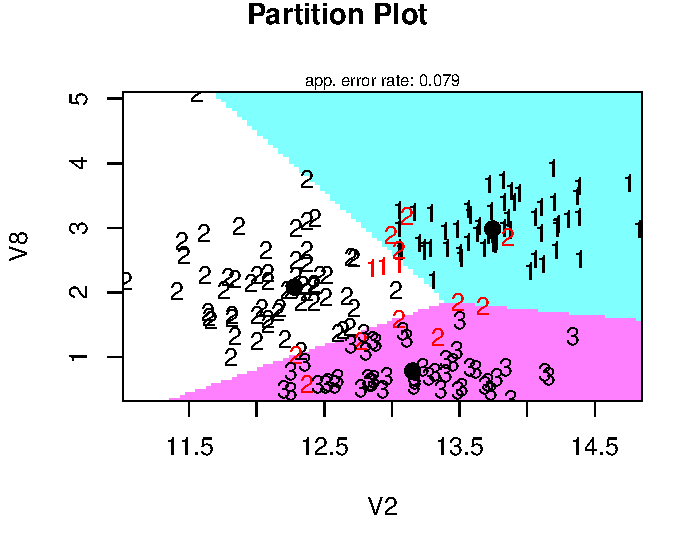
\includegraphics[width=\maxwidth]{figure/unnamed-chunk-12} 

}


\begin{kframe}\begin{alltt}
\hlcom{# b)}

\hlstd{zt} \hlkwb{<-} \hlkwd{numeric}\hlstd{(}\hlnum{1010}\hlstd{)}
\hlkwa{for}\hlstd{(i} \hlkwa{in} \hlnum{1}\hlopt{:}\hlnum{1010}\hlstd{)\{}
  \hlstd{zt[i]} \hlkwb{<-} \hlnum{1}\hlopt{/}\hlnum{1000}\hlopt{*}\hlstd{i} \hlopt{+} \hlstd{xt[i]}
\hlstd{\}}

\hlstd{z_tren} \hlkwb{<-} \hlkwd{ts}\hlstd{(zt[}\hlnum{1}\hlopt{:}\hlnum{1000}\hlstd{])}
\hlstd{z_test} \hlkwb{<-} \hlkwd{ts}\hlstd{(zt[}\hlnum{1001}\hlopt{:}\hlnum{1010}\hlstd{],}\hlkwc{start}\hlstd{=}\hlnum{1001}\hlstd{,}\hlkwc{end}\hlstd{=}\hlnum{1010}\hlstd{)}

\hlcom{# c)}

\hlkwd{plot}\hlstd{(z_tren,}\hlkwc{type}\hlstd{=}\hlstr{"l"}\hlstd{)}
\end{alltt}
\end{kframe}

{\centering \includegraphics[width=\maxwidth]{figure/unnamed-chunk-13} 

}


\begin{kframe}\begin{alltt}
\hlkwd{acf}\hlstd{(z_tren)}
\end{alltt}
\end{kframe}

{\centering \includegraphics[width=\maxwidth]{figure/unnamed-chunk-14} 

}


\begin{kframe}\begin{alltt}
\hlcom{# widoczny jest trend}

\hlcom{# d)}

\hlstd{ztd} \hlkwb{<-} \hlkwd{diff}\hlstd{(z_tren)}
\hlkwd{ts.plot}\hlstd{(ztd)}
\end{alltt}
\end{kframe}

{\centering \includegraphics[width=\maxwidth]{figure/unnamed-chunk-15} 

}


\begin{kframe}\begin{alltt}
\hlkwd{acf}\hlstd{(ztd)}
\end{alltt}
\end{kframe}

{\centering \includegraphics[width=\maxwidth]{figure/unnamed-chunk-16} 

}


\begin{kframe}\begin{alltt}
\hlkwd{pacf}\hlstd{(ztd)}
\end{alltt}
\end{kframe}

{\centering \includegraphics[width=\maxwidth]{figure/unnamed-chunk-17} 

}


\begin{kframe}\begin{alltt}
\hlcom{# po roznicowaniu jest duzo lepiej}

\hlcom{# e)}

\hlcom{# proponuj� ARMA(3,4)}

\hlstd{model_moj} \hlkwb{<-} \hlkwd{arima}\hlstd{(ztd,} \hlkwd{c}\hlstd{(}\hlnum{3}\hlstd{,}\hlnum{0}\hlstd{,}\hlnum{4}\hlstd{))}
\hlkwd{Box.test}\hlstd{(model_moj}\hlopt{$}\hlstd{resid,}\hlkwc{lag}\hlstd{=}\hlnum{20}\hlstd{,}\hlkwc{type}\hlstd{=}\hlstr{"Ljung"}\hlstd{)}
\end{alltt}
\begin{verbatim}
## 
## 	Box-Ljung test
## 
## data:  model_moj$resid
## X-squared = 12.62, df = 20, p-value = 0.8931
\end{verbatim}
\begin{alltt}
\hlcom{# funkcja ar() dopasowuje nam model AR i sama wybiera rzad modelu:}

\hlstd{model_ar} \hlkwb{<-} \hlkwd{ar}\hlstd{(ztd,} \hlkwc{aic}\hlstd{=}\hlnum{TRUE}\hlstd{,} \hlkwc{method}\hlstd{=}\hlstr{"mle"}\hlstd{,} \hlkwc{order.max}\hlstd{=}\hlkwa{NULL}\hlstd{)}

\hlstd{model_ar}\hlopt{$}\hlstd{order}        \hlcom{# rzad}
\end{alltt}
\begin{verbatim}
## [1] 4
\end{verbatim}
\begin{alltt}
\hlstd{model_ar}\hlopt{$}\hlstd{ar}           \hlcom{# wspolczynniki}
\end{alltt}
\begin{verbatim}
## [1]  0.07479 -0.60409  0.12627 -0.07081
\end{verbatim}
\begin{alltt}
\hlstd{model_ar}\hlopt{$}\hlstd{x.mean}       \hlcom{# wyraz wolny}
\end{alltt}
\begin{verbatim}
## [1] 0.0009581
\end{verbatim}
\begin{alltt}
\hlkwd{Box.test}\hlstd{(model_ar}\hlopt{$}\hlstd{resid,}\hlkwc{lag}\hlstd{=}\hlnum{20}\hlstd{,}\hlkwc{type}\hlstd{=}\hlstr{"Ljung"}\hlstd{)}   \hlcom{# moj model byl lepszy :D}
\end{alltt}
\begin{verbatim}
## 
## 	Box-Ljung test
## 
## data:  model_ar$resid
## X-squared = 27.87, df = 20, p-value = 0.1125
\end{verbatim}
\begin{alltt}
\hlcom{# f)}

\hlstd{aic} \hlkwb{<-} \hlkwd{matrix}\hlstd{(}\hlnum{0}\hlstd{,}\hlnum{7}\hlstd{,}\hlnum{7}\hlstd{)}
\hlstd{bic} \hlkwb{<-} \hlkwd{matrix}\hlstd{(}\hlnum{0}\hlstd{,}\hlnum{7}\hlstd{,}\hlnum{7}\hlstd{)}

\hlkwa{for}\hlstd{(p} \hlkwa{in} \hlnum{0}\hlopt{:}\hlnum{6}\hlstd{)\{}
   \hlkwa{for}\hlstd{(q} \hlkwa{in} \hlnum{0}\hlopt{:}\hlnum{6}\hlstd{)\{}
      \hlstd{model} \hlkwb{<-} \hlkwd{arima}\hlstd{(ztd,} \hlkwd{c}\hlstd{(p,}\hlnum{0}\hlstd{,q),}\hlkwc{method}\hlstd{=}\hlstr{"ML"}\hlstd{,}
                     \hlkwc{optim.control}\hlstd{=}\hlkwd{list}\hlstd{(}\hlkwc{maxit}\hlstd{=}\hlnum{10}\hlopt{^}\hlnum{5}\hlstd{))}
      \hlstd{aic[p}\hlopt{+}\hlnum{1}\hlstd{,q}\hlopt{+}\hlnum{1}\hlstd{]} \hlkwb{<-} \hlkwd{AIC}\hlstd{(model)}
      \hlstd{bic[p}\hlopt{+}\hlnum{1}\hlstd{,q}\hlopt{+}\hlnum{1}\hlstd{]} \hlkwb{<-} \hlkwd{AIC}\hlstd{(model,}\hlkwc{k}\hlstd{=}\hlkwd{log}\hlstd{(}\hlnum{1000}\hlstd{))}
   \hlstd{\}}
\hlstd{\}}

\hlstd{wym_aic} \hlkwb{<-} \hlkwd{which}\hlstd{(aic}\hlopt{==}\hlkwd{min}\hlstd{(aic),}\hlkwc{arr.ind}\hlstd{=}\hlnum{TRUE}\hlstd{)}\hlopt{-}\hlnum{1}
\hlstd{wym_bic} \hlkwb{<-} \hlkwd{which}\hlstd{(bic}\hlopt{==}\hlkwd{min}\hlstd{(bic),}\hlkwc{arr.ind}\hlstd{=}\hlnum{TRUE}\hlstd{)}\hlopt{-}\hlnum{1}

\hlstd{wym_aic}
\end{alltt}
\begin{verbatim}
##      row col
## [1,]   6   1
\end{verbatim}
\begin{alltt}
\hlstd{wym_bic}
\end{alltt}
\begin{verbatim}
##      row col
## [1,]   4   2
\end{verbatim}
\begin{alltt}
\hlstd{model_aic} \hlkwb{<-} \hlkwd{arima}\hlstd{(ztd,}\hlkwd{c}\hlstd{(wym_aic[}\hlnum{1}\hlstd{],}\hlnum{0}\hlstd{,wym_aic[}\hlnum{2}\hlstd{]))}
\hlstd{model_bic} \hlkwb{<-} \hlkwd{arima}\hlstd{(ztd,}\hlkwd{c}\hlstd{(wym_bic[}\hlnum{1}\hlstd{],}\hlnum{0}\hlstd{,wym_bic[}\hlnum{2}\hlstd{]))}

\hlkwd{Box.test}\hlstd{(model_aic}\hlopt{$}\hlstd{resid,}\hlkwc{lag}\hlstd{=}\hlnum{20}\hlstd{,}\hlkwc{type}\hlstd{=}\hlstr{"Ljung"}\hlstd{)}
\end{alltt}
\begin{verbatim}
## 
## 	Box-Ljung test
## 
## data:  model_aic$resid
## X-squared = 11.86, df = 20, p-value = 0.9209
\end{verbatim}
\begin{alltt}
\hlkwd{Box.test}\hlstd{(model_bic}\hlopt{$}\hlstd{resid,}\hlkwc{lag}\hlstd{=}\hlnum{20}\hlstd{,}\hlkwc{type}\hlstd{=}\hlstr{"Ljung"}\hlstd{)}
\end{alltt}
\begin{verbatim}
## 
## 	Box-Ljung test
## 
## data:  model_bic$resid
## X-squared = 23.58, df = 20, p-value = 0.261
\end{verbatim}
\begin{alltt}
\hlcom{# model_aic wyglada na najlepszy ze wszystkich}

\hlcom{# g)}

\hlstd{pr_bic} \hlkwb{<-} \hlkwd{predict}\hlstd{(model_bic,}\hlkwc{n.ahead}\hlstd{=}\hlnum{10}\hlstd{)}\hlopt{$}\hlstd{pred}
\hlstd{se_bic} \hlkwb{<-} \hlkwd{predict}\hlstd{(model_bic,}\hlkwc{n.ahead}\hlstd{=}\hlnum{10}\hlstd{)}\hlopt{$}\hlstd{se}

\hlkwd{ts.plot}\hlstd{(pr_bic,} \hlkwd{diff}\hlstd{(z_test), pr_bic} \hlopt{+} \hlnum{2}\hlopt{*}\hlstd{se_bic, pr_bic} \hlopt{-} \hlnum{2}\hlopt{*}\hlstd{se_bic,}
        \hlkwc{col}\hlstd{=}\hlkwd{c}\hlstd{(}\hlstr{"red"}\hlstd{,}\hlstr{"black"}\hlstd{,}\hlstr{"red"}\hlstd{,}\hlstr{"red"}\hlstd{),} \hlkwc{lty}\hlstd{=}\hlkwd{c}\hlstd{(}\hlnum{1}\hlstd{,}\hlnum{1}\hlstd{,}\hlnum{3}\hlstd{,}\hlnum{3}\hlstd{),} \hlkwc{main}\hlstd{=}\hlstr{"BIC"}\hlstd{)}
\end{alltt}
\end{kframe}

{\centering \includegraphics[width=\maxwidth]{figure/unnamed-chunk-18} 

}


\begin{kframe}\begin{alltt}
\hlstd{pr_aic} \hlkwb{<-} \hlkwd{predict}\hlstd{(model_aic,}\hlkwc{n.ahead}\hlstd{=}\hlnum{10}\hlstd{)}\hlopt{$}\hlstd{pred}
\hlstd{se_aic} \hlkwb{<-} \hlkwd{predict}\hlstd{(model_aic,}\hlkwc{n.ahead}\hlstd{=}\hlnum{10}\hlstd{)}\hlopt{$}\hlstd{se}

\hlkwd{ts.plot}\hlstd{(pr_aic,} \hlkwd{diff}\hlstd{(z_test), pr_aic} \hlopt{+} \hlnum{2}\hlopt{*}\hlstd{se_aic, pr_aic} \hlopt{-} \hlnum{2}\hlopt{*}\hlstd{se_aic,}
        \hlkwc{col}\hlstd{=}\hlkwd{c}\hlstd{(}\hlstr{"red"}\hlstd{,}\hlstr{"black"}\hlstd{,}\hlstr{"red"}\hlstd{,}\hlstr{"red"}\hlstd{),} \hlkwc{lty}\hlstd{=}\hlkwd{c}\hlstd{(}\hlnum{1}\hlstd{,}\hlnum{1}\hlstd{,}\hlnum{3}\hlstd{,}\hlnum{3}\hlstd{),} \hlkwc{main}\hlstd{=}\hlstr{"AIC"}\hlstd{)}
\end{alltt}
\end{kframe}

{\centering \includegraphics[width=\maxwidth]{figure/unnamed-chunk-19} 

}


\begin{kframe}\begin{alltt}
\hlstd{pr_ar} \hlkwb{<-} \hlkwd{predict}\hlstd{(model_ar,}\hlkwc{n.ahead}\hlstd{=}\hlnum{10}\hlstd{)}\hlopt{$}\hlstd{pred}
\hlstd{se_ar} \hlkwb{<-} \hlkwd{predict}\hlstd{(model_ar,}\hlkwc{n.ahead}\hlstd{=}\hlnum{10}\hlstd{)}\hlopt{$}\hlstd{se}

\hlkwd{ts.plot}\hlstd{(pr_ar,} \hlkwd{diff}\hlstd{(z_test), pr_ar} \hlopt{+} \hlnum{2}\hlopt{*}\hlstd{se_ar, pr_ar} \hlopt{-} \hlnum{2}\hlopt{*}\hlstd{se_ar,}
        \hlkwc{col}\hlstd{=}\hlkwd{c}\hlstd{(}\hlstr{"red"}\hlstd{,}\hlstr{"black"}\hlstd{,}\hlstr{"red"}\hlstd{,}\hlstr{"red"}\hlstd{),} \hlkwc{lty}\hlstd{=}\hlkwd{c}\hlstd{(}\hlnum{1}\hlstd{,}\hlnum{1}\hlstd{,}\hlnum{3}\hlstd{,}\hlnum{3}\hlstd{),} \hlkwc{main}\hlstd{=}\hlstr{"AR"}\hlstd{)}
\end{alltt}
\end{kframe}

{\centering \includegraphics[width=\maxwidth]{figure/unnamed-chunk-110} 

}


\begin{kframe}\begin{alltt}
\hlcom{# h)}

\hlstd{blad_ar} \hlkwb{<-} \hlkwd{sum}\hlstd{((pr_ar[}\hlopt{-}\hlnum{1}\hlstd{]} \hlopt{-} \hlkwd{diff}\hlstd{(z_test))}\hlopt{^}\hlnum{2}\hlstd{)}
\hlstd{blad_bic} \hlkwb{<-} \hlkwd{sum}\hlstd{((pr_bic[}\hlopt{-}\hlnum{1}\hlstd{]} \hlopt{-} \hlkwd{diff}\hlstd{(z_test))}\hlopt{^}\hlnum{2}\hlstd{)}
\hlstd{blad_aic} \hlkwb{<-} \hlkwd{sum}\hlstd{((pr_aic[}\hlopt{-}\hlnum{1}\hlstd{]} \hlopt{-} \hlkwd{diff}\hlstd{(z_test))}\hlopt{^}\hlnum{2}\hlstd{)}

\hlstd{blad_ar}
\end{alltt}
\begin{verbatim}
## [1] 0.2323
\end{verbatim}
\begin{alltt}
\hlstd{blad_bic}
\end{alltt}
\begin{verbatim}
## [1] 0.2351
\end{verbatim}
\begin{alltt}
\hlstd{blad_aic}
\end{alltt}
\begin{verbatim}
## [1] 0.2382
\end{verbatim}
\begin{alltt}
\hlcom{# i)}

\hlstd{model_true} \hlkwb{<-} \hlkwd{arima}\hlstd{(}\hlkwd{diff}\hlstd{(z_tren),}\hlkwd{c}\hlstd{(}\hlnum{3}\hlstd{,}\hlnum{0}\hlstd{,}\hlnum{2}\hlstd{),}\hlkwc{include.mean}\hlstd{=}\hlnum{TRUE}\hlstd{)}
\hlstd{model_true}\hlopt{$}\hlstd{coef}
\end{alltt}
\begin{verbatim}
##        ar1        ar2        ar3        ma1        ma2  intercept 
## -0.6407516 -0.5900645 -0.2775594  0.7204050  0.0366392  0.0009614
\end{verbatim}
\begin{alltt}
\hlcom{# zgadzaja sie z teoretycznymi :D}

\hlkwd{Box.test}\hlstd{(model_ar}\hlopt{$}\hlstd{resid,}\hlkwc{lag}\hlstd{=}\hlnum{20}\hlstd{,}\hlkwc{type}\hlstd{=}\hlstr{"Ljung"}\hlstd{)}
\end{alltt}
\begin{verbatim}
## 
## 	Box-Ljung test
## 
## data:  model_ar$resid
## X-squared = 27.87, df = 20, p-value = 0.1125
\end{verbatim}
\begin{alltt}
\hlkwd{Box.test}\hlstd{(model_bic}\hlopt{$}\hlstd{resid,}\hlkwc{lag}\hlstd{=}\hlnum{20}\hlstd{,}\hlkwc{type}\hlstd{=}\hlstr{"Ljung"}\hlstd{)}
\end{alltt}
\begin{verbatim}
## 
## 	Box-Ljung test
## 
## data:  model_bic$resid
## X-squared = 23.58, df = 20, p-value = 0.261
\end{verbatim}
\begin{alltt}
\hlkwd{Box.test}\hlstd{(model_aic}\hlopt{$}\hlstd{resid,}\hlkwc{lag}\hlstd{=}\hlnum{20}\hlstd{,}\hlkwc{type}\hlstd{=}\hlstr{"Ljung"}\hlstd{)}
\end{alltt}
\begin{verbatim}
## 
## 	Box-Ljung test
## 
## data:  model_aic$resid
## X-squared = 11.86, df = 20, p-value = 0.9209
\end{verbatim}
\begin{alltt}
\hlkwd{Box.test}\hlstd{(model_true}\hlopt{$}\hlstd{resid,}\hlkwc{lag}\hlstd{=}\hlnum{20}\hlstd{,}\hlkwc{type}\hlstd{=}\hlstr{"Ljung"}\hlstd{)}
\end{alltt}
\begin{verbatim}
## 
## 	Box-Ljung test
## 
## data:  model_true$resid
## X-squared = 23.15, df = 20, p-value = 0.2817
\end{verbatim}
\end{kframe}
\end{knitrout}


\end{document}
